\newpage
% ~\\
% \newpage

\section{Prior reviews}
\label{appendix:past-reviews}

This paper has been submitted to IEEE Symposium on Security and Privacy 2020.

We thank and really appreciate the reviewers who took time to provide us with
such detailed feedback.

\subsection{S\&P 2020 Review \#582A}

Overall merit: 3. Weak reject - The paper has flaws, but I will
not argue against it.

\begin{center}
  \subheading{===== Brief paper summary (2-3 sentences) =====}
\end{center}

This paper presents a verification of the C implementation
of the X25519 key-exchange protocol in the TweetNaCl
library. Correctness properties including the C code implements
the algorithm correctly are verified in Coq, using the
Verified Software Toolchain (VST).


\begin{center}
  \subheading{===== Strengths =====}
\end{center}

+ This paper produces a fully formally verified crypto library.

+ This paper presents solid technical work.


\begin{center}
  \subheading{===== Weaknesses =====}
\end{center}

- The novelty of this paper is not well explained. It’s unclear
whether this paper has pushed the boundary in terms of what
can be formally verified.


\begin{center}
  \subheading{===== Detailed comments for the author(s) =====}
\end{center}

I appreciate work on producing fully verified software. This
paper presents another instance: X25519 protocol. The result
here is very strong: it verified both safety properties and the
correctness of the C implementation.

One main weakness of this paper is that it is hard to extract
from the writing, what are the new discoveries in this
exercise. Are there new proof techniques developed for this
verification? Is there anything new about the way that loops
are handled? Is the application of reflection challenging? Are
there bugs found, in particular, in the mathematical operations?

\begin{answer}{EEEEEE}
The novelty of this work is not in the proof techniques. It
lies in the assurance gained by the formalization of the
X25519 from RFC 7748, and its correctness with respect to
the theory of elliptic curves. Additionally it is the first
time, a link from the C code up to the mathematical definitions of
Curve25519 using a single tool is presented.
\end{answer}

A related comment is that it is unclear from the paper
whether now we can re-use proofs in this paper to verify
mathematical operations of other protocols that use elliptic
curve.

\begin{answer}{EEEEEE}
We believe that parts of our proofs are reusable either by
their structure to give an intuition or by directly changing
some values (for e.g. X448). The mathematical definitions
are generic and may be instantiated over any fields (of characteristic
neither 2 or 3). The Ladder may be instantiated
over operations over different data structure for the underlying
arithmetic, making it reusable. The low level operations
\eg \TNaCle{A} are also reusable in the proof of ed25519.
\end{answer}

In the Corrections in TweetNaCl paragraph, two things
were discussed. It’s unclear how and whether either one of
them directly relate to the verification effort. It would be nice
if they are. Then the story for the usefulness of the verification
become stronger.

\begin{answer}{EEEEEE}
The switch from \TNaCle{i64} to \TNaCle{int} in \texttt{for} loops and the
extraction of the computation outside of the function call in
\TNaCle{pack25519} are required by VST but we believe those
change have no impact on the verification effort.

The only modification which made the verification easier
was the removal of the \textit{dead code} at the end of
\TNaCle{crypto_scalarmult}. Peter Wu and Jason A.
Donenfeld had also noticed this part and informed us after we
already fixed the code.
\end{answer}

It would be nice if the authors comment on the verification
effort: person month etc.

\begin{answer}{EEEEEE}
In addition to the time required to get familiar with
research software, we faced a few bugs which we reported
to the developers of VST to get them fixed.
It is very hard to work with a tool without being involved
in the development loop. Additionally newer versions often
broke some of our proofs and it was often needed to adapt
to the changes.
As a result we do not believe the metric person-month to be
a good representation of the verification effort.
\end{answer}

Also, did the verified version replace the version in use in
production software? If not, why not?

\begin{answer}{EEEEEE}
We contacted the authors of TweetNaCl and expect that
the changes above mentioned will soon be integrated in a
new version of the library, mostly for \TNaCle{car25519} and the
simplification in \TNaCle{crypto_scalarmult}.
\end{answer}

Section V is extremely dry. What are the high-level insights?
Perhaps a picture representation of how the theorems
and lemmas fit together would be a better way to represent
this section.

\begin{answer}{EEEEEE}
We provided overviews of the proof at the beginning of sections
V.1 and V.2. We hope this will give the reader an intuition
of how lemmas fit together.
\end{answer}

In summary, this paper is in need of significant improvements
in the writing and providing detailed discussions of
high-level intellectual contributions in this verification effort.

{\color{gray}
Minor

On page 6: "each elements" => no s

On page 7, the beginning of the page, a half sentence is
dangling there.

On page 9: "each functions" => no s}


\subsection{S\&P 2020 Review \#582B}

Overall merit: 4. Weak accept - While flawed, the paper has
merit and we should consider accepting it.


\begin{center}
  \subheading{===== Brief paper summary (2-3 sentences) =====}
\end{center}

In this paper, the authors verify the C implementation of the
X25519 elliptic curve key exchange in the TweetNaCl library,
a short implementation of the NaCl library. The X25519 key
exchange method is used in TLS 1.3, Signal, Tor, Zcash and
SSH. Within TLS 1.3 (and probably also in other protocols),
any implementation of X25519 may be used in an implementation
of the standard. Thus, the present work contributes
to a fully verified code-base for TLS 1.3 (and other crucial
protocols)

The verification itself is practically significant. The paper
makes a good effort to describe the approach, but I was, at
times, a little disappointed at the description. Performing this
type of verification yields substantial human understanding
and enables the authors to carry out a similar approach for
other primitives much more easily. I wish that the authors
would extract their conceptual insights on the technique and
communicate those to the readers. Regardless, I would very
much like to see this work at S\&P, but I would like to encourage
the authors to de-emphasize technical details (even more)
and spend more space of the body on conceptual insights (see
comments below).


\begin{center}
  \subheading{===== Detailed comments for the author(s) =====}
\end{center}

I was confused that you did not seem have found any errors
in an implementation. I can believe that the implementers
of \cite{BGJ+15} are proficient implementers, but I would have expected
some minor bugs/parsing issues to be found anyway. What is
your explanation that you haven’t found any issues?

\begin{answer}{EEEEEE}
The implementation of TweetNaCl is straight forward and
simple, big number arithmetic is done without optimizations.
It is easy to get an intuition of how the code work by reading
it. The ladder is a direct mapping of RFC~7748. It does
not aim for speed optimizations. This reduce significantly
the complexity of the code compared to e.g., Fiat Crypto
generated optimized C code.

While we did not find errors in the implementation with
respect to functional correctness under the CompCert assumptions,
we removed an undefined behavior by the C
standard.
\end{answer}

p.1: You discuss \cite{Ber06} as using heavy annotation of code,
differently from your own code. However, as far as I understand,
your Coq implementation must also be type-annotated. Thus,
I imagine that the difference lies in whether SAT-solvers are
used or not? This did not become very clear, because you
mostly describe names of tool while leaving out the details of
what these tools carry out conceptually.

\begin{answer}{EEEEEE}
SMT solvers strategies are in need of annotation, often written
as parsable comment in the middle of the C code~\cite{acsl}
in order to ``guide'' the proof. In our case we only need to
annotate the beginning of the function and loop invariants
which allows us to get tighter bounds.
\end{answer}

p.2: Fig 1 is very nice. However, at this point, none of
the notation has been explained to the reader, and I imagine
that V stands for VST? It wasn't clear to me. Maybe, the
caption of the figure could explain what the details inside the
figures represent. In particular, the Figure seems to used a
nice abstraction of properties that is not used elsewhere in
the paper. I.e., elsewhere in the paper, there is usually a lot
of code details.

\begin{answer}{EEEEEE}
``.V'' is the file extension for Coq files (as opposed to ``.C'' for C
files). This allows us to emphasis that all our work is done
in a single framework. We clarified this in the introduction.
\end{answer}

p.2-4: Subsection A took some mathematical background.
Obviously, not all of it could be covered, but the motivation
for why certain content was presented and not others was not
clear to me as a reader, which was quite frustrating. In Section
B, it was even less clear why particular details were presented,
e.g., the discussion of the computation of n’ was completely
unclear to me. Subsection D seemed a good idea, but was very
tough to follow, too much content in short time. Subsection D
seems to jump between implementation levels and discussing
high-level arguments such as Fermat’s little theorem.

\begin{answer}{EEEEEE}
We aim to give a quick view of how Montgomery curves are
defined and remind the reader of the ``twisting factor''. The
computation of n' is required for the security of X25519 as
it reduces the computations to a prime-order group, we use
this presentation to refer it later as ``clamping''. We
modified Subsection D to omit all the code definitions of small
functions to ease the reader experience. The C definitions
are now provided in the appendix.
\end{answer}

p.3: I very much liked the discussion of the Diff between
TweetNaCl and your modifications! I imagine that many of
them are conceptually interesting in that they make verification
easier. I would have enjoyed reading a conceptual discussion
of the differences. Instead, Appendix A just contains a
Diff, and as a reader, I would need to perform the extraction
of insights myself.

\begin{answer}{EEEEEE}
Due to page restrictions for IEEE S\&P, including appendices,
We had a condensed diff. We changed the format to
a ``diff -u'' to provide the context of the applied changes. We
also now describe the motivations of each changes below
the said Diff.
\end{answer}

p.5: CSWAP: Maybe use a backward reference to p.3 where
CSWAP was defined, since in between, there was a lot of
content, and relying on the reader's memory does not really
work here (or at least, it did not work for me).

\begin{answer}{EEEEEE}
As we rewrote significantly section 2.4, the space between
the definition and the use of CSWAP decreased. We added a
backward reference to where it was originally defined.
\end{answer}

p.7: I enjoyed the discussion on aliasing! This was the type
of conceptual discussion I find interesting. I was confused
about the mentioning that the case distinction k=0,1,2 does
not cover "all cases" - all cases of what? And why is this
distinction sufficient for the task at hand?

\begin{answer}{EEEEEE}
In that section we clarified the discussion of what
would be an unnecessary aliasing case and why such case do
not happen in TweetNaCl. For example, TweetNaCl never
has function calls where the 3 pointers are aliased (\texttt{o = a = b}),
as such we do not consider this aliasing case in the
specifications of the function.
\end{answer}

Most of the rest of the paper felt hard to read, because it
read like a chronological enumeration of all steps. I think that
it would be much more interesting if the paper highlights the
interesting aspects of the verification.

\begin{answer}{EEEEEE}
We removed sections and details in order to simplify the
reading experience. We also added figures in section V in
order to provide the reader a mental image of how the lemmas,
definitions and theorems work together.
\end{answer}

Related work:

\newcommand{\rbar}{\cite{DBLP:journals/corr/BhargavanDFHPRR17}}

In reference \rbar, the order of authors is different than
in the original publication. I think that you might want to
discuss \rbar in the Related work section, since it seems quite
close. I was wondering whether you consider the approach
in \rbar as synthesis or verification, because to me, it seemed
a mix/neither.

\begin{answer}{EEEEEE}
The bibtex was from DBLP. We fixed the order of the
authors with respect to the original publication and contacted
DBLP to update their files.

\fref{tikz:LowVST} highlights the difference between Low*
and our approach.

\begin{figure}[H]
\centering
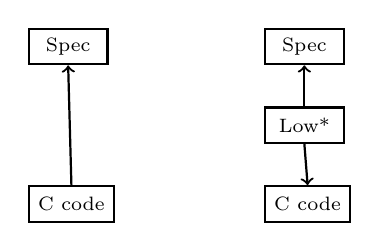
\begin{tikzpicture}[textstyle/.style={black, thick, anchor=north west, align=center, minimum height=0.45cm, minimum width=1cm, text centered, font=\scriptsize}]
  \node [textstyle,draw] (VSTSpec) at (0,0) {Spec};
  \node [textstyle,draw] (VSTC) at (0,-2) {C code};
  \draw [->, thick] (VSTC.north) -- (VSTSpec.south);

  \begin{scope}[yshift=0 cm,xshift=3 cm]
    \node [textstyle,draw] (LowSpec) at (0,0) {Spec};
    \node [textstyle,draw] (Low) at (0,-1) {Low*};
    \node [textstyle,draw] (LowC) at (0,-2) {C code};
    \draw [->, thick] (Low.south) -- (LowC.north);
    \draw [->, thick] (Low.north) -- (LowSpec.south);
  \end{scope}
\end{tikzpicture}

\caption{VST vs Low*}
\label{tikz:LowVST}
\end{figure}

Low* generates C code, thus this is synthesis. We generate
Clight from C code, thus this is verification. Because Low*
also has a verification step with respect to some high-level
specifications, we consider their process to be a mix of the
two methods. Also to be noted that both VST and Low*
allow the verification of memory safety.
% However Low* provides
% sidechannel securities while VST allow verification
% of concurent programs.
\end{answer}

Clarification in intro:

The intro states that this is, to the authors knowledge, the
first use of Verifiable Software Toolchain (VST) in software
verification of an implementation of an asymmetric cryptographic
primitives. Does this mean that VST has been used
for symmetric cryptographic primitives before? From the text,
I wasn’t sure whether this is careful quantification or not.

\begin{answer}{EEEEEE}
This is indeed careful quantification. VST has already
been used to verify symmetric Cryptographic primitives
(\eg SHA), as mentioned later by \cite{Beringer2015VerifiedCA} and \cite{2015-Appel}.
\end{answer}


\subsection{S\&P 2020 Review \#582C}

Overall merit: 3. Weak reject - The paper has flaws, but I will
not argue against it.


\begin{center}
  \subheading{===== Brief paper summary (2-3 sentences) =====}
\end{center}

This paper presents a formalization of the X25519
(Curve25519) elliptic curve Diffie-Hellman (ECDH)
construction in Coq, and uses this formalization to verify the
functional correctness of a C implementation of this
construction taken from the TweetNaCl library. Going further than
prior work, the authors also link their Coq specification to a
mathematical theory of elliptic curves in Coq.


\begin{center}
  \subheading{===== Strengths =====}
\end{center}

Proofs of cryptographic algorithms like X25519 tend to
mean different things in different communities: (a) one may
prove that X25519 implements a group based on the mathematical
theory of elliptic curves, (b) one may prove that an
X25519 implementation meets its mathematical spec, or (c)
one may prove that a protocol that uses X25519 is provably
secure, based on some cryptographic assumption on the ECDH
construction. It is rare to find papers that combine more than
one of these proof levels, and this paper does a creditable
job of linking (a) with (b), relying on the Coq framework to
soundly glue these proofs together. Although a similar goal
was considered in \cite{Zinzindohoue2016AVE}, this paper provides a more satisfying
solution by not leaving any gaps between the formalizations,
and by relying on a smaller trusted computing base.


\begin{center}
  \subheading{===== Weaknesses =====}
\end{center}

X25519 implementations have now been verifying in multiple
papers using multiple verification frameworks, and \cite{Erbsen2016SystematicSO}
even uses Coq to verify a large portion of a C implementation
of X25519 fully automatically. So, the main contribution
here is that that the authors verify an existing popular
implementation (TweetNaCl) without making many changes to
the source code. Still, TweetNaCl is not necessarily the most
complex (and certainly not the most efficient) implementation
of X25519 that has been verified, which makes the novelty of
this work hard to justify.

\newcommand{\mitp}{\cite{Erbsen2016SystematicSO}}


\begin{answer}{EEEEEE}
Indeed \mitp's C code of X25519 is verified. However the
authors do not qualify their approach as verification but
as synthesis. They do not use Coq to verify C code, instead they
``synthesize'' (generate) C code from verified refinements of
the specification. Our approach goes from the C code up to the
specification.
 % which is completely different.

\begin{figure}[H]
\centering
\begin{tikzpicture}[textstyle/.style={black, thick, anchor=north west, align=center, minimum height=0.45cm, minimum width=2.5cm, text centered, font=\small}]
  \begin{scope}[yshift=0 cm,xshift=0 cm]
    \node [textstyle] (our) at (0,0.635) {Our paper};
    \node [textstyle,draw] (VSTSpec) at (0,0) {Spec};
    \node [textstyle,draw] (VSTC) at (0,-1.5) {\textit{Verified} C code};
    \draw [-{Latex[length=3mm]}, double, thick] (VSTC.north) -- (VSTSpec.south) node [midway, below, textstyle, anchor=west] {\textbf{Verification}};
  \end{scope}

  \begin{scope}[yshift=0 cm,xshift=4 cm]
    \node [textstyle] (mit) at (0,0.635) {\mitp};
    \node [textstyle,draw] (MITSpec) at (0,0) {Spec};
    \node [textstyle,draw] (MITC) at (0,-1.5) {\textit{Verified} C code};
    \draw [-{Latex[length=3mm]}, double, thick] (MITSpec.south) -- (MITC.north) node [midway, below, textstyle, anchor=west] {\textbf{Synthesis}};
  \end{scope}
\end{tikzpicture}

\caption{Our approach vs \mitp}
\label{tikz:MitVST}
\end{figure}

\end{answer}


\begin{center}
  \subheading{===== Detailed comments for the author(s) =====}
\end{center}

I like the approach taken in this paper and I think this work
has value and should be published. However, I am not sure
the current presentation of the work works well.

The paper can be essentially divided into two components:
the proof of TweetNaCl using VST, and the proof of equivalence
between the Coq spec of RFC7748 and the mathematical
theory of Curve25519. The details of both are interesting
to formalists but the Coq details are quite hard to parse and
distracting when trying to understand the text. This is a well-known
problem for formal verification papers, and I don’t
have great advice except to suggest that the authors separate
out the code fragments into figures and let the text focus on
the high-level ideas of the code.

\begin{answer}{EEEEEE}
We removed a significant part of the Coq details, especially
details about reflections in order to make the reading
experience smooth. As suggested, we also added a few figures to
give the reader an overview of how the proofs are linked
together.
\end{answer}

At the end of Section IV, I would have loved to see some
high-level lessons on what the proof taught you, and what
part of this proof would be reusable if you decided to verify
Ed25519 or X448 or P-256, for example. This is particularly
important for this work, since prior papers have shown how
to share proof effort across multiple curves.

\begin{answer}{EEEEEE}
We added insights in \sref{subsec:with-VST} of how to improve
working with VST. In section \sref{sec:Conclusion},
we described in further details how our work can
be extended to other curves. The TweetNaCl ed25519
implementation makes use of the same low level arithmetic
as X25519, reusing our proofs. For example, \TNaCle{pow2523} is
similar to \TNaCle{inv25519} and would allow us to reuse our
reflection abstraction. X448 would reuse the ladder but the
low level arithmetic would need to be proven again. P-256
is a different case as due to its short Weierstra\ss{} shape, this
implies that our ladder is not fit for it. However using \cite{BartziaS14}
and our proofs as example it is possible to prove a similar
ladder as ours.
\end{answer}

It also appears that the authors do not verify the constant-time
guarantees of the TweetNaCl code. Could this be done
in their framework?

\begin{answer}{EEEEEE}
Constant-timeness is not a property verifiable with VST.
This is not verifiable with our framework.
% Related on CompCert: https://eprint.iacr.org/2019/926.pdf
\end{answer}

Section V presents the proof of mathematical equivalence.
It appears to me that this proof is completely independent of
the TweetNaCl proof. Is that the case? Is there any lemma
from the first part that is needed in the second? More
importantly, could you claim that your proof of equivalence also
provides a justification for the implementations of Fiat Crypto
or HACL*, hence adding value to those other projects in addition
to your own?

\begin{answer}{EEEEEE}
Indeed those two proofs are completely independent. The
only link between \sref{sec:C-Coq} and \sref{sec:maths} is the definition
of \Coqe{RFC} and the preconditions on the inputs: 2 arrays of
32 bytes. We highlighted in \sref{sec:Conclusion} that our proof of
correctness of X25519 in RFC~7748 increases the confidence
in other implementations such as Fiat Crypto and HACL*
(under the assumption they correctly formalized the RFC).
\end{answer}

I was hoping to see where the ``clamping'' used in X25519
would appear in the formalization of Section V but was unable
to spot it. Does clamping affect the proofs in any way? Is there
a stronger property you could prove because of the clamping
(e.g. membership in the prime-order group)? Do you already
prove such a property?

\begin{answer}{EEEEEE}
The clamping by itself has no impact on the computations using the ladder.
It is thus normal to not see it appear in \sref{sec:maths} as our proofs work for any 255-bit $n$,
We prove the correctness of X25519 in RFC~7748, we do not prove its security.
The proof of a stronger property (e.g. membership in prime-order group)
shall be done separately before being applied to Curve25519.
\end{answer}

More generally, what about the proof of Section V is
specific to X25519 and what is generic?

\begin{answer}{EEEEEE}
Everything in \sref{subsec:ECC} is generic, anything left in \sref{subsec:curve_twist_fields}
is specific to X25519.
\end{answer}
